%Ch2.GeneralPointSetTopology.tex
\ifx\allfiles\undefined
\documentclass{ctexrep}
\usepackage{amsmath}
\usepackage{amssymb}
\usepackage{amsthm}
\usepackage{amsfonts}
\usepackage{mathrsfs}
\usepackage{enumitem}
\usepackage{braket}
\usepackage{hyperref}


\newcommand{\pare}[1]{\left(#1\right)}
\newcommand{\blr}[1]{\left[#1\right)}
\newcommand{\lbr}[1]{\left(#1\right]}
\newcommand{\brac}[1]{\left[#1\right]}
\newcommand{\curb}[1]{\left\{#1\right\}}
\newcommand{\abs}[1]{\left|\, #1 \,\right|}
\newcommand{\rec}[1]{\frac{1}{#1}}
\newcommand{\N}{\mathbb{N}}
\newcommand{\Q}{\mathbb{Q}}
\newcommand{\Z}{\mathbb{Z}}
\newcommand{\R}{\mathbb{R}}
\newcommand{\unk}{\mathcal{X}}
\newcommand{\bu}[3]{#1_{#2}^{\pare{#3}}}
\newcommand{\dref}[1]{定义\ref{def:#1}}
\newcommand{\tref}[1]{定理\ref{thm:#1}}
\newcommand{\lref}[1]{引理\ref{lem:#1}}
\newcommand{\cref}[1]{推论\ref{coll:#1}}
\newcommand{\pref}[1]{命题\ref{prp:#1}}
\newcommand{\func}[3]{#1:\, #2 \rightarrow #3}
\newcommand{\overbar}[1]{\mkern 1.5mu\overline{\mkern-1.5mu#1\mkern-1.5mu}\mkern 1.5mu}
\newcommand{\clo}[1]{\overbar{#1}}
\newcommand{\supi}[2]{\overbar{\int_{#1}^{#2}}}
\newcommand{\infi}[2]{\underbar{\int_{#1}^{#2}}}
\newcommand{\setf}{\mathscr}
\newcommand{\bool}{\mathrm{bool}}
\newcommand{\inc}{++}
\newcommand{\defeq}{:=}
\newcommand{\ntuple}{$n$元组}
\newcommand{\card}[1]{\#\pare{#1}}
\newcommand{\setcond}[2]{\curb{#1 \, \left| \, #2 \right.}}
\newcommand{\setcondl}[2]{\curb{\left. #1 \, \right| \, #2}}
\newcommand{\bv}[1]{\mathbf{#1}}
\newcommand{\bfa}{\bv{a}}
\newcommand{\bfb}{\bv{b}}
\newcommand{\bfx}{\bv{x}}
\newcommand{\bfy}{\bv{y}}
\newcommand{\bfe}{\bv{e}}
\newcommand{\bfF}{\bv{F}}
\newcommand{\bff}{\bv{f}}
\newcommand{\bfG}{\bv{G}}
\newcommand{\bfH}{\bv{H}}
\newcommand{\bfg}{\bv{g}}
\newcommand{\bfh}{\bv{h}}
\newcommand{\bfr}{\bv{r}}
\newcommand{\bfk}{\bv{k}}
\newcommand{\bfu}{\bv{u}}
\newcommand{\bfv}{\bv{v}}
\newcommand{\oo}[1]{o\pare{#1}}
\newcommand{\OO}[1]{O\pare{#1}}
\newcommand{\norm}[1]{\left\| #1 \right\|}
\newcommand{\DD}{\mathbf{D}}
\newcommand{\comp}{\circ}
\newcommand{\const}{\mathrm{const}}
\newcommand{\dist}[2]{d\pare{#1,#2}}
\newcommand{\len}{\ell}
\newcommand{\siga}{$\sigma$-代数}
\newcommand{\cara}{Carath\'{e}odory}
\newcommand{\Gd}{G_\delta}
\newcommand{\Fs}{F_\sigma}
\newcommand{\mmani}{$m$-维流形}
\newcommand{\open}[1]{\mathcal{#1}}
\newcommand{\half}{\frac{1}{2}}
\newcommand{\maxo}[1]{\text{max}\curb{#1}}
\newcommand{\mino}[1]{\text{min}\curb{#1}}
\newcommand{\epsclo}{$\epsilon$-接近}
\newcommand{\close}[1]{$#1$-接近}
\newcommand{\cinf}{$C^\infty$}
\newcommand{\cuno}{$C^1$}
\newcommand{\Int}{\text{Int}\,}
\newcommand{\Ext}{\text{Ext}\,}
\newcommand{\funcf}{\mathcal}
\newcommand{\DDu}{\overbar{\DD}}
\newcommand{\DDl}{\underbar{\DD}}
\newcommand{\Diff}[1]{\mathrm{Diff}_{#1}\,}
\newcommand{\Av}[1]{\mathrm{Av}_{#1}\,}
\newcommand{\Lip}[1]{Lipschitz-$#1$}
\newcommand{\sgn}[1]{\mathrm{sgn}}
\newcommand{\eset}{\varnothing}
\newcommand{\cT}{\mathcal{T}}
\newcommand{\cS}{\mathcal{S}}
\newcommand{\cG}{\mathcal{G}}
\newcommand{\cF}{\mathcal{F}}
\newcommand{\cC}{\mathcal{C}}
\newcommand{\cB}{\mathcal{B}}

\newcommand{\hd}{H\"{o}lder}

\renewcommand{\proofname}{证明}

\newenvironment{cenum}{\begin{enumerate}\itemsep0em}{\end{enumerate}}

\newtheorem{definition}{定义}[section]
\newtheorem{lemma}{引理}[section]
\newtheorem{theorem}{定理}[section]
\newtheorem{collary}{推论}[section]
\newtheorem{proposition}{命题}[section]
\newtheorem{axiom}{公理}[section]
\newtheorem{ex}{例}[section]

\newenvironment{aenum}{\begin{enumerate}[label=\textnormal{(\alph*)}]}{\end{enumerate}}
\begin{document}
\fi

%Content

\chapter{普通点集拓扑}
  \section{拓扑空间与连续函数}
  \subsection{拓扑空间}
  \begin{definition}
  集合$X$上的一个拓扑$\cT$谓$X$的一满足如下条件的子集族:
  \begin{cenum}
    \item $\curb{\eset, X} \in \cT$;
    \item $\cT$中元素的任意并仍在$\cT$中;
    \item $\cT$中元素的有限交仍在$\cT$中。
  \end{cenum}
  \end{definition} 
  \begin{definition}
  $X$的所有子集构成的拓扑谓离散拓扑。
  \end{definition}
  \begin{definition}
  由$X$和$\eset$构成的拓扑谓密着拓扑。
  \end{definition}
  \begin{definition}
  由$X$本身与所有满足$X-U$为有限集的$U$构成的拓扑谓有限补拓扑。
  \end{definition}
  \begin{definition}
  $\cT'\supset\cT$则$\cT'$细于$\cT$,反之则谓粗于。
  \end{definition}
  如果把开集比做石子,把石子打碎就得到更细的拓扑。
  \subsection{拓扑的基}
  \begin{definition}
  \label{def:tb}
  基$\cB$谓满足如下条件的子集族:
  \begin{cenum}
    \item 对任意$x\in X$,存在$B\in\cB$满足$x\in B$;
    \item 对任意$x\in B_1\cap B_2$,存在$B$满足$x\in B$且$B\subset B_1\cap B_2$。
  \end{cenum}
  \end{definition}
  注意此定义不针对具体的拓扑。
  \begin{ex}
  平面上的圆域和矩形域构成的集族都构成基。
  \end{ex}
  \begin{definition}
  满足\dref{tb}的$\cB$生成的拓扑为所有满足对$x\in U$,存在$x\in B\subset U$的$U$的集族。
  \end{definition}
  可以直接验证上述定义构成一个拓扑。对所有$x$取对应的$x\in B_x$后将诸$B_x$并起,可得等价的表述
  \begin{theorem}
  若$\cB$为$\cT$的基,则$\cT$为$\cB$中元素并的族。
  \end{theorem}
  \begin{theorem}
  设$\cC$为开集族,若对于任意开集$U$中任意$x$,存在$C\in\cC$满足$x\in C\subset U$,则$\cC$为$\cT$的基。
  \end{theorem}
  \begin{proof}
  容易验证$\cC$为基。再分别证$\cC\subset \curb{U}$与$\curb{\cup C}\supset \curb{U}$。
  \end{proof}
  \begin{theorem}
  \label{thm:critfiner}
  设$\cB$于$\cB'$分别生成$\cT$与$\cT'$,则$\cT'$细于$\cT$当且仅当对任意$x\in B$存在$x\in B'\subset B$。
  \end{theorem}
  \begin{proof}
  强行带入定义,即任意$U$均在$\cT'$内即可。
  \end{proof}
  \begin{definition}
  $\R$上的$\pare{a,b}$生成的拓扑谓标准拓扑。
  \end{definition}
  \begin{definition}
  $\R$上$\blr{a,b}$生成的拓扑谓下限拓扑,记作$\R_\ell$。
  \end{definition}
  \begin{definition}
  $\R$上$\pare{a,b}$与$\pare{a,b} - \curb{\rec{n}}$生成的拓扑谓K-拓扑,记作$\R_K$。
  \end{definition}
  \begin{lemma}
  $\R_\ell$与$\R_K$严格细于标准拓扑,但它们之间不可比较。
  \end{lemma}
  \begin{proof}
  $\R_K$\emph{严格}细于的证明只需考虑$x=0$与$B=\pare{-1,1}-\curb{1/n}$,同一个集合可证$\R_\ell$不细于$R_K$。
  \end{proof}
  \begin{definition}
  子基$\cS$谓满足$\cup S=X$的集族。
  \end{definition}
  \begin{definition}
  子基生成的拓扑谓$\cS$中有限交的所有并。
  \end{definition}
  可以直接验证$\curb{\cap S}$为一个基,故其确实生成一拓扑。
  \subsection{序拓扑}
  \begin{definition}
  具有全序关系的$X$上的序拓扑谓所有$\pare{a,b}$,$\lbr{a,\max X}$,$\blr{\min X, b}$生成的拓扑。
  \end{definition}
  \begin{ex}
  $\Z_+$上的序拓扑是离散拓扑。然而$X=\curb{1,2}\times\Z_+$的字典序拓扑下单点集$1\times1$并非开集。
  \end{ex}
  \begin{definition}
  全序集$X$中$a$决定的射线谓开射线$\pare{a,+\infty}$,$\pare{-\infty,a}$,$\blr{a,+\infty}$,$\lbr{-\infty,a}$。
  \end{definition}
  所有开射线构成$X$的序拓扑的子基。
  \subsection{积拓扑}
  \begin{definition}
  $X\times Y$上的积拓扑谓所有$U\times V$的集族$\cB$生成的拓扑,其中$U$与$V$为$X$与$Y$中的开集。
  \end{definition}
  \begin{theorem}
  若$\cB$与$\cC$分别为$X$与$Y$的基,则$\cB\times\cC$为$X\times Y$的基。
  \end{theorem}
  \begin{definition}
  投射$\pi_1\pare{x,y}=x$,$\pi_2\pare{x,y}=y$。
  \end{definition}
  \begin{theorem}
  如下的$\cS$构成$X\times Y$的一子基,其中$U$和$V$分别为$X$与$Y$中的开集。
  \[ \cS = \curb{\pi_1^{-1}\pare{U}}\cup\curb{\pi_2^{-1}\pare{V}}. \]
  \end{theorem}
  \subsection{子空间拓扑}
  \begin{definition}
  对$X$的子集$Y$定义子空间拓扑,其中$U$为$X$中的开集。
  \[ \cT_Y = \curb{Y\cap U}. \]
  \end{definition}
  \begin{theorem}
  若$\cB$为$X$的一个基,则
  \[ \cB_Y = \setcond{B\cap Y}{B \in \cB} \]
  谓$Y$的子空间拓扑的一个基。
  \end{theorem}
  \begin{lemma}
  若$Y$为$X$中开集而$U$为$Y$中开集,则$U$为$X$中开集。
  \end{lemma}
  \begin{theorem}
  若$A\subset X$,$B\subset Y$,则$A\times B$的积拓扑与其自$X\times Y$继承的子空间拓扑相符。
  \end{theorem}
  然而,对于序拓扑无类似结论。
  \begin{ex}
  考虑$X=\R$而$Y=\brac{0,1}$,$Y$上的序拓扑与子空间拓扑相符。
  \end{ex}
  \begin{ex}
  考虑$X=\R$而$Y=\blr{0,1}\cup\curb{2}$,子空间拓扑中$\curb{2}$为开集,二者不符。
  \end{ex}
  \begin{ex}
  考虑$X=\R^2$而$Y=\brac{0,1}\times\brac{0,1}$,则$\half\times\lbr{\half,1}$为子空间拓扑的开集但不是序拓扑的开集。
  \end{ex}
  \begin{definition}
  子集$Y$称为凸的,如果对$Y$中$a<b$皆有$\pare{a,b}\subset Y$。
  \end{definition}
  \begin{theorem}
  设$X$为全序集,$Y$为凸子集,则子空间拓扑与序拓扑一致。
  \end{theorem}
  \begin{proof}
  借助开射线构造子基后证明其相互包含即可。
  \end{proof}
  \subsection{闭集与极限点}
  \begin{definition}
    若$X-A$为开集,则$A$为闭集。
  \end{definition}
  \begin{ex}
  $\R$中$\brac{a,b}$为闭集,$\R^2$中$\R_+^2$为闭集,有限补拓扑中$X$、$\eset$、有限集为闭集。
  \end{ex}
  \begin{ex}
  离散拓扑每一个集合都是开集也都是闭集,$Y=\brac{0,1}\cup\pare{2,3}$中两个分量都同时是开集和闭集。
  \end{ex}
  \begin{definition}
  对于拓扑空间$X$,成立
  \begin{cenum}
    \item $\eset$、$X$都是闭集;
    \item 闭集的任意交仍为闭集;
    \item 闭集的有限并仍为闭集。
  \end{cenum}
  \end{definition} 
  \begin{theorem}
    $A$为$X$的子空间$Y$的闭集当且仅当有闭集$C$满足$A=Y\cap C$。
  \end{theorem}
  \begin{theorem}
    $A$是$Y$的闭集,$Y$是$X$的闭集,则$A$是$X$的闭集。
  \end{theorem}
  \subsubsection{Hausdorff空间}
  \begin{definition}
    集合的内部$\inter{A}$是包含于其内的所有开集的并,闭包$\clo{A}$是其外所有闭集的交。
  \end{definition}
  显然开集的内部是本身,闭集的闭包也是本身。注意$\pare{0,1}$在其本身中的闭包和在$\R$中的闭包不同,所称闭包都是指父空间闭包。
  \begin{theorem}
  $Y$中$\clo{A}^Y = \clo{A} \cap X$。
  \end{theorem}
  \begin{definition}
    两集合相交,如果它们的交非空。
  \end{definition}
  \begin{definition}
    含有$x$的开集称为其邻域。
  \end{definition}
  \begin{theorem}
  \label{thm:sublpoint}
    $x\in \clo{A}$当且仅当每一个邻域与$A$相交。
  \end{theorem}
  \begin{proof}
    如果存在反例$U$,则$X-U$会成为包含$A$的闭集。
  \end{proof}
  \begin{collary}
    $x\in \clo{A}$当且仅当含有$x$的每一个基元素与$A$相交。
  \end{collary}
  \begin{ex}
    $A=\lbr{0,1}$,$\clo{A}=\brac{0,1}$。$A=\Q$,$\clo{A}=\R$。$\clo{\curb{1/n}} = \curb{1/n}\cup\curb{0}$。
  \end{ex}
  \subsubsection{极限点}
  \begin{definition}
    若$x$的任何一个邻域包含$A$中其他点,则$x$为$A$的极限点。
  \end{definition}
  \begin{ex}
    $A=\lbr{0,1}$,$\brac{0,1}$中的点均为其极限点。$A=\Q$,$\R$中的点均为其极限点。$A=\curb{1/n}$,$0$为其极限点。
  \end{ex}
  \begin{theorem}
  \label{thm:closureeq}
  $\clo{A} = A\cup A'$,其中$A'$为极限点集合。
  \end{theorem}
  \begin{proof}
    参考\tref{sublpoint}。
  \end{proof}
  \begin{collary}
  $A$为闭集当且仅当$A'\subset A$。
  \end{collary}
  \subsubsection{Hausdorff空间}
  \begin{definition}
    \label{def:converge}
    如果\forest{$x$的任意邻域$U$}{$N$}{当$n>N$,$x_n\in U$},则$\curb{x_n}$收敛到点$x$。
  \end{definition}
  $\R^2$和$\R$中的序列最多收敛至一点,然而其他拓扑空间不一定。
  \begin{definition}
    若$X$中任意两不同点存在无交邻域,则称$X$为一Hausdorff空间(Hausdorff space)。
  \end{definition}
  \begin{theorem}
    Hausdorff空间中有限集为闭集。
  \end{theorem}
  \begin{proof}
    只证单点集。由于隔离邻域的存在,易见其他点都不在闭包内。
  \end{proof}
  比Hausdorff条件更弱的,有\tuno 。
  \begin{definition}
    若$X$中有限集为闭,则$X$满足\tuno 。
  \end{definition}
  \begin{theorem}
    若$X$满足\tuno ,则$x$为$A$的极限点当且仅当$x$的任意邻域与$A$有无限交点。
  \end{theorem}
  \begin{proof}
    如果有一个邻域只有有限交点,挖掉还是开集,但不再与$A$相交。
  \end{proof}
  \begin{theorem}
    \label{thm:hausonepoint}
    若$X$为Hausdorff空间,则$X$中的序列最多收敛至一点。
  \end{theorem}
  \begin{proof}
    如果有两个点,在定义中取隔离邻域即可。
  \end{proof}
  \begin{theorem}
  每一个具有序拓扑的全序集,两个Hausdorff空间的积,Hausdorff空间的子空间是Hausdorff空间。
  \end{theorem}
  \begin{proof}
    全序集可选取中间元分割,中间元不存在的直接射线可分割。
  \end{proof}
  \subsection{连续函数}
  \subsubsection{函数的连续性}
  \begin{definition}
    函数$\func{f}{X}{Y}$称为连续的,如果开集的原像为开集。
  \end{definition}
  为了证明函数连续,只需要证明基的原像为开集即可。
  \begin{ex}
  \label{ex:epsd}
    上述定义等价于$\epsilon-\delta$定义。
  \end{ex}
  \begin{proof}
    如果$\epsilon-\delta$定义成立,则$f\pare{x}$的$\epsilon$-邻域的原像包含$x$的$\delta$-邻域,故任意开集的原像均为开集。如果拓扑定义成立,则显而易见。
  \end{proof}
  \begin{ex}
    $\func{f}{\R}{\R_\ell}$的$f\pare{x}=x$不是连续函数,但其逆连续。
  \end{ex}
  \begin{theorem}
  \label{thm:contineq}
    对于$\func{f}{X}{Y}$,下列条件等价:
    \begin{cenum}
      \item $f$连续;
      \item 对$X$的任意子集$A$有$f\pare{\clo{A}}\subset\clo{f\pare{A}}$;
      \item 对$Y$中任意闭集$B$有$f^{-1}\pare{B}$为闭集;
      \item 对任意$x$与$f\pare{x}$的邻域$V$,存在$x$的邻域$U$满足$f\pare{U}\subset{V}$。
    \end{cenum}
  \end{theorem}
  \begin{proof}
    $1\Rightarrow 2$:若$y$在$f\pare{A}$外一开集内,则原像为$f\pare{A}$外一开集。$2\Rightarrow 3$:闭集$f\pare{A} = \clo{f\pare{A}}\supset f\pare{\clo{A}}$,故$A=\clo{A}$。$3\Rightarrow 1$与$1\Rightarrow 4 \Rightarrow1$显然。
  \end{proof}
  \subsubsection{同胚}
  \begin{definition}
    如果一个一一映射和它的逆都连续,则称之为同胚。
  \end{definition}
  \begin{definition}
    如果$X$的性质于与之同胚的$Y$都成立,则称之为拓扑性质。
  \end{definition}
  \begin{definition}
    映入子空间的同胚称为嵌入。
  \end{definition}
  \begin{ex}
    $F\pare{x}=x/\pare{1-x^2}$与$G\pare{y}=2y/\pare{1+\pare{1+4y^2}^{1/2}}$为$\pare{-1,1}$与$\R$间同胚。
  \end{ex}
  \begin{ex}
    \label{ex:01tocircle}
    $\blr{0,1}$弯曲到圆周的映射连续而非同胚。其扩张连续而非嵌入。
  \end{ex}
  \subsubsection{构造连续函数}
  \begin{theorem}
    \label{thm:continauscontin}
    下列函数皆连续:
    \begin{cenum}
      \item 常值函数;
      \item 子空间到父空间的内射;
      \item 连续函数的复合;
      \item 连续函数限制定义域到一子空间的结果;
      \item 连续函数限制或扩大值域至包含像集的子空间或父空间的结果;
      \item 若$X$可写为开集的并,且$f$在每个分量上连续。
    \end{cenum}
  \end{theorem}
  \begin{theorem}[黏结引理]
    设$X=A\cup B$且二者为闭集,并且$\func{f}{A}{Y}$与$\func{g}{B}{Y}$连续且在$A\cap B$上相等,则$h$连续,
    \[ h\pare{x}=\begin{cases}f\pare{x}, x\in A, \\ g\pare{x}, x\in B.\end{cases} \]
  \end{theorem}
  \begin{proof}
    由\tref{contineq},注意闭集被映回闭集即可。
  \end{proof}
  \begin{ex}
    对$x\ge 0$,$h\pare{x}=x$,$x\le 0$,$h\pare{x}=x/2$,则$h$连续。
  \end{ex}
  \begin{theorem}
    \label{thm:continprod}
    $\func{f}{A}{X\times Y}$连续的充分必要条件为$f_X$与$f_Y$连续。
  \end{theorem}
  \begin{proof}
    注意连续的拓扑定义等价于对基连续即可。
  \end{proof}
  \begin{ex}
    \label{ex:veccontin}
    向量场连续当且仅当分量连续。
  \end{ex}
  \subsection{积拓扑}
  \begin{definition}
    $X$的元素的$J$-串为$\func{\vx}{J}{X}$,其全体记作$X^J$。
  \end{definition}
  例如,$\R^3\isom \R^{\curb{1,2,3}}$。
  \begin{definition}
    $A_j$的笛卡尔积$\prod A_j$为各取一元构成之$J$-串的集合。
  \end{definition}
  \begin{definition}
    基由$\prod U_\alpha$构成$\prod X_\alpha$的称为箱拓扑。
  \end{definition}
  \begin{definition}
    子基由$\curb{\pi^{-1}\pare{U_{\alpha}}}$构成的称为积拓扑。
  \end{definition}
  \begin{theorem}
    箱拓扑的基由所有$\prod U_\alpha$构成,积拓扑的基由$\prod U_\alpha$构成但$U_\alpha$中只有有限个非$X_\alpha$。
  \end{theorem}
  \begin{theorem}
    $\prod B_\alpha$构成箱拓扑的积,$\prod B_\alpha$中若$B_\alpha$中只有有限个非$X_\alpha$则构成积拓扑的基。
  \end{theorem}
  \begin{ex}
    $\R^n$的积拓扑与箱拓扑一致。
  \end{ex}
  \begin{theorem}
    $\prod A_\alpha$在两种拓扑下都是$\prod X_\alpha$的同种拓扑的子空间。
  \end{theorem}
  \begin{theorem}
    若每个$X_\alpha$都是Hausdorff的,则两拓扑下$\prod X_\alpha$都如此。
  \end{theorem}
  \begin{theorem}
    在$\prod X_\alpha$的两种拓扑下都有$\prod \clo{A_\alpha} = \clo{\prod A_\alpha}$。
  \end{theorem}
  \begin{proof}
    若$x$在$\prod \clo{A_\alpha}$内,则诸$\prod U_\alpha$均有$\prod A_\alpha$的元素,故$x$在$\clo{\prod A_\alpha}$内。若$x$在$\prod \clo{A_\alpha}$外$U_\alpha$内,则$\pi^{-1}\pare{U_\alpha}$包含$x$且为开集,故在$\clo{\prod A_\alpha}$外。
  \end{proof}
  \begin{theorem}
    积拓扑下$\func{f}{A}{\prod X_\alpha}$连续当且仅当各个分量连续。
  \end{theorem}
  \begin{proof}
    注意连续的拓扑定义等价于对基成立即可。
  \end{proof}  
  \begin{ex}
    对箱拓扑下$\R$的可数无限积$\R^\omega$,$f\pare{t}=\pare{t,t,t,\cdots}$不连续。注意$\pare{-1,1}\times\pare{-1/2,1/2}\times\pare{-1/3,1/3}$被映回$0$即可。
  \end{ex}
  \subsection{度量拓扑}
  \begin{definition}
    集合$X$的一个度量$d$是一个函数$\func{d}{X\times X}{\R}$,满足正定、对称与三角不等式。
  \end{definition}
  \begin{definition}
    以全体$\epsilon$-球为基的拓扑称为度量拓扑。
  \end{definition}
  容易验证全体$\epsilon$-球构成基。由这一定义,开集可视作满足任意$y\in U$都有某$B\pare{x,\epsilon}\subset U$的集合$U$。
  \begin{ex}
    若$x=y$,$d\pare{x,y}=1$,否则$d\pare{x,y}=0$诱导出离散拓扑。
  \end{ex}
  \begin{ex}
    $d\pare{x,y}=\abs{x-y}$诱导$\R$上的序拓扑。
  \end{ex}
  \begin{definition}
    若$X$的拓扑由某度量诱导,则称$X$为度量空间。
  \end{definition}
  \begin{definition}
    度量空间的子集$A$为有界的,若$d\pare{a_1,a_2}$一致有界。$A$的直径谓$\diam A = \sup\curb{d\pare{a_1,a_2}}$。
  \end{definition}
  \begin{theorem}
    \label{thm:sbmeqm}
    由度量$d$诱导的度量
    \[ \sbm{d}\pare{x,y} = \min\curb{d\pare{x,y}, 1} \]
    谓标准有界度量,它和$d$诱导同一拓扑。
  \end{theorem}
  \begin{proof}
    分类验证三角不等式即可。
  \end{proof}
  \begin{definition}
    对$\R^n$中的点,$d\pare{\vx,\vy} = \norm{\vx-\vy} = \pare{\sum\pare{x_i-y_i}^2}^{1/2}$诱导欧氏度量,$\rho\pare{\vx,\vy} = \max\curb{\abs{x_i-y_i}}$诱导平方度量。
  \end{definition}
  欧式度量的三角不等式是熟知的结论。平方度量由
  \[ d_3 = \abs{x_k-z_k} \le \abs{x_k-y_k} + \abs{y_k-z_k} \le d_1 + d_2 \]
  验证三角不等式。注意同理可证若$X$上度量$d_1$和$Y$上度量$d_2$可以生成$X\times Y$上一度量$d_3 = \max\curb{d_1,d_2}$。
  \par
  欧式度量和平方度量的基元素分别为圆域和方域。由\tref{critfiner}立得
  \begin{theorem}
    度量拓扑$\cT'$细于$\cT$当且仅当对于任意$x$与$\epsilon$,存在$\epsilon'$满足
    \[ B'\pare{x,\epsilon'} \subset B\pare{x, \epsilon}. \]
  \end{theorem}
  \begin{theorem}
    \label{thm:eucsqreq}
    欧氏度量和平方度量诱导$\R^n$上的积拓扑。
  \end{theorem}
  \begin{proof}
    直接验证不难,但由$\rho \le r \le \sqrt{n} \rho$可立得欧式与平方拓扑等价。
  \end{proof}
  \begin{definition}
    对$\R^J$中的点定义
    \[ \rho\pare{\vx,\vy} = \sup\setcond{\sbm{d}\pare{x_\alpha,y_\alpha}}{\alpha\in J}, \]
    可得一致度量,诱导出一致拓扑。
  \end{definition}
  \begin{theorem}
    一致拓扑细于积拓扑,粗于箱拓扑。$J$为无限集则两两不同。
  \end{theorem}
  \begin{proof}
    玩弄基元素的大小可证其粗细。$J$无限时,$\pare{-1,1}^J$在一致拓扑下为开,积拓扑下非开。$\prod \pare{-1/n,1/n}$在箱拓扑下为开,一致拓扑下非开。
  \end{proof}
  \begin{theorem}
    \label{thm:metricprodR}
    对$\R$的可数无限积$\R^\omega$定义
    \[ D\pare{\vx, \vy} = \sup\curb{\frac{\sbm{d}\pare{x_i,y_i}}{i}}, \]
    可诱导$\R^\omega$上的积拓扑。
  \end{theorem}
  \begin{proof}
    设$\R^\omega$的某基$B$的分量在$j$后均为$\R$,则某$B\pare{x, \epsilon/j}$包含其内。反之也可以选择这样的基包含于$B\pare{x, 1/j}$内。
  \end{proof}
  类似证明可仿照得到
  \begin{theorem}
    可度量化空间的可数积仍可度量化。
  \end{theorem}
  \begin{ex}
    在$X\times Y=\R^2$上定义$d=\min\curb{y_2-y_1,1}$,如果两点共$x$,否则$d = 1+\pare{x_1-x_2}$,则$d$诱导字典序拓扑。
  \end{ex}
  \begin{ex}
    易见度量空间的子空间仍为度量空间,且子空间的度量直接限制定义域可得。
  \end{ex}
  \subsection{连续函数与度量拓扑}
  \begin{theorem}
    \label{thm:contineqdeltaepsilon}
    度量空间到度量空间的$\func{f}{X}{Y}$的连续性等价于$\epsilon$-$\delta$条件。
  \end{theorem}
  \begin{proof}
    仿照\eref{epsd}可得。
  \end{proof}
  \begin{corollary}
  \label{coll:metricscontin}
    度量为连续函数。
  \end{corollary}
  \begin{lemma}[序列引理]
    \label{lem:seq}
    若$A$中有收敛于$x$的序列,则$x\in\clo{A}$。若$X$为度量空间,逆命题成立。
  \end{lemma}
  \begin{theorem}
    \label{thm:matricscontineq}
    度量空间之间的$\func{f}{X}{Y}$连续的充要条件谓$x_n\rightarrow x$等价于$f\pare{x_n}\rightarrow f\pare{x}$。
  \end{theorem}
  \begin{proof}
    若拓扑条件成立,则$f\pare{x}$的小邻域原像都会包含$x$的邻域,故包含$\curb{x_n}_{n\ge N}$。若序列条件成立,结合序列引理与\tref{contineq}即可。
  \end{proof}
  注意上述定理对满足下列条件的空间也可以直接适用。
  \begin{definition}
    如果$x$有邻域$\curb{U_n}$满足任意邻域$U$都有某$U_n$含于其内,则称$X$在$x$处有可数基。如果处处都有则称$X$满足第一可数性公理。
  \end{definition}
  \begin{lemma}
    \label{lem:asmd}
    加减乘除是其定义域内的连续函数。
  \end{lemma}
  \begin{theorem}
    \label{thm:continasmd}
    连续函数加减乘的结果连续,恒非零的除亦连续。
  \end{theorem}
  \begin{definition}
    若$\curb{f_n}$关于度量$d\pare{f,g}=\sup\curb{\abs{f-g}}$收敛于$f$,则称其一致收敛。
  \end{definition}
  \begin{theorem}
    \label{thm:uniformconvergecontin}
    一致收敛的连续函数列收敛于连续函数。
  \end{theorem}
  \begin{proof}
    对给定的$\epsilon$,存在$\delta$和$N$使得当$\abs{x-y}<\delta$,诸变差皆小于$\delta$。
    \[ \abs{f\pare{x}-f\pare{y}} \le \abs{f\pare{x}-f_N\pare{x}} +  \abs{f_N\pare{x}-f_N\pare{y}} +  \abs{f\pare{y}-f_N\pare{y}}.\qedhere\]
  \end{proof}
  \begin{collary}
    若$x_n\rightarrow x$而$\curb{f_n}$一致收敛于$f$,则$f_n\pare{x_n}\rightarrow f\pare{x}$。
  \end{collary}
  \begin{ex}
    箱拓扑的$\R^\omega$不满足序列引理因此不可度量化。$0\in\clo{\R_+^\omega}$但$\prod\pare{-x_{ii},x_{ii}}$排斥所有$x_i$。
  \end{ex}
  \begin{ex}
    不可数个$\R$的积空间不可度量化。
  \end{ex}
  \begin{proof}
    考虑$\R^J$由那些知有有限个零分量的$\curb{0,1}$序列的子空间,易见$0$在其内。然而,能有幸为零的分量指标仅有可数个,故存在恒$1$的指标。
  \end{proof}
  \subsection{商拓扑}
  \begin{definition}
    满射$\func{p}{X}{Y}$称为商映射,如果$U$是$Y$的开集当且仅当$\inv{p}\pare{U}$是$X$的开集。
  \end{definition}
  易见开集也可以改为闭集。
  \begin{definition}
    $X$的子集$C$为饱和的,如果它是纤维的并。
  \end{definition}
  商映射等价于饱和开集映射到开集。易见开映射和闭映射(把开集映射到开集或者把闭集映射到闭集)都是商映射。
  \begin{ex}
    $\brac{0,1}\cup\brac{2,3}$到$\brac{0,2}$的黏贴映射是闭映射但不是开映射。
  \end{ex}
  \begin{ex}
    $\func{\pi_1}{\R\times\R}{\R}$是开映射但不是闭映射,因为$\curb{y=1/x}$被映射到开集。
  \end{ex}
  \begin{ex}
  \label{ex:qnotoc}
    $\pi_1$在$A=\R\times0 \cup \blr{0,\infty} \times \R$上的限制是商映射,但不是开映射或者闭映射。$A-\lbr{-\infty,0}\times 0$是开集,但是被映射到闭集。$\curb{y=\pm\tan x}$图像左侧是闭集,但被映射到开集。
  \end{ex}
  \begin{definition}
    满射$\func{p}{X}{A}$的像$A$上存在一拓扑使得$X$为商映射,此拓扑谓商拓扑。
  \end{definition}
  \begin{ex}
    $y=\sgn\pare{x}$在点集上可以诱导一个商拓扑$\curb{\curb{\curb{-1},\curb{1}},0}$。
  \end{ex}
  \begin{definition}
    $X^*$为$X$的分拆,则$\func{\pi}{X}{X^*}$诱导的商拓扑使$X^*$为商空间。
  \end{definition}
  \begin{ex}
    将单位圆盘将圆周视为等价类,则商空间同胚于球面。
  \end{ex}
  \begin{ex}
    将矩形四角和对边上对应点视为等价类,则商空间同胚于环面。
  \end{ex}
  由\eref{qnotoc}知商映射在子空间的限制未必是商映射,但仍然有
  \begin{theorem}
    设商映射$\func{p}{X}{Y}$与饱和子空间$A$,则$p$在其上的限制$\func{q}{A}{p\pare{A}}$仍为商映射,如果
    \begin{cenum}
      \item $A$为开集或闭集;
      \item 或者$p$为开映射或闭映射。
    \end{cenum}
  \end{theorem}
  \begin{proof}
    先验证,如果$V\subset p\pare{A}$,则$\inv{q}\pare{V} = \inv{p}\pare{V}$。如果$U\subset X$,则$p\pare{U\cap A}=p\pare{U}\cap p\pare{A}$。都有$\inv{q}\pare{V}$是开的$\Rightarrow V$在$p\pare{A}$中为开。
  \end{proof}
  商映射的复合仍为商映射,但乘积不一定,Hausdorff空间的商空间也不一定是Hausdorff空间。
  \begin{theorem}
    商映射$p$与纤维上的映射$g$诱导$f$满足$f\comp p=g$。$f$连续当且仅当$g$连续,$f$为商映射当且仅当$g$为商映射。
  \end{theorem}
  \centerline{\xymatrix{
      X\ar[d]_p\ar[dr]^g \\
      Y\ar@{.>}[r]_f & Z
    }}{}
  \begin{proof}
    若$p$和$g$为商映射,证明$\inv{f}\pare{V}$为开集$\Rightarrow V$为开集即可。
  \end{proof}
  \begin{corollary}
    设$\func{g}{X}{Z}$为连续满射,$X^*$为各纤维的集,取商拓扑,则
    \begin{cenum}
      \item $g$诱导的$\func{f}{X^*}{Z}$一一连续,其为同胚当且仅当$g$为商映射;
      \item 若$Z$为Hausdorff空间,则$X^*$为Hausdorff空间。
    \end{cenum}
  \end{corollary}
  \centerline{\xymatrix{
      X\ar[d]_p\ar[dr]^g \\
      X^*\ar[r]_f & Z
    }}{}
  \begin{proof}
    注意一一的商映射等价于同胚。
  \end{proof}
  \begin{ex}
    设$X=\brac{0,1}\times\curb{1,2,\cdots}$,$Z=x\times \pare{x/n}$其中$x\in\brac{0,1}$,则$g\pare{x\times n} = x\times\pare{x/n}$诱导出$X^*$为将$X$诸左端点粘合的空间,但$\func{f}{X^*}{Z}$不是同胚。
  \end{ex}
  \begin{proof}
    考虑$x_n=\pare{1/n}\times n$,则$\curb{x_n}$为闭集但是$z_n=\pare{1/n}\times{1/n^2}$不是,因此$g$不是商映射。
  \end{proof}
  \begin{ex}
    设$\func{p}{X}{X^*}$是将$\R$的$\Z_+$粘合为$b$形成的商空间,$\func{i}{\Q}{\Q}$为恒等映射,则$p\times i$不是商映射。
  \end{ex}
  \begin{proof}
    假设$U_n$为$n\times\pare{\sqrt{2}/n}$附加其上方和下方的条带,$U=\cup U_n$,则$U$饱和但$p\times i\pare{U}$不是开集,因为某$I_b\times I_\delta$的原像包含条带的缝隙。
  \end{proof}
  \section{连通性与紧致性}
  \subsection{连通空间}
  \begin{definition}
    拓扑空间$X$的一个分割,谓其一对无交非空开集其并为$X$。
  \end{definition}
  \begin{lemma}
    若$Y$是$X$的子空间,则其分割的分量彼此不包含对方的极限点。若存在一对并为$Y$的非空集合彼此不包含对方极限点,则亦构成分割。
  \end{lemma}
  \begin{proof}
    注意分量既开又闭,故极限点自含。若存在这样的一对,则$A$中任意元素都存在小邻域在$B$外,故在$A$内,故$A$为开集。
  \end{proof}
  \begin{ex}
    密着拓扑是连通的。
  \end{ex}
  \begin{ex}
    $\R$的子空间$\blr{-1,0}\cup\lbr{0,1}$不是连通的。
  \end{ex}
  \begin{ex}
    $\Q$不是连通的。
  \end{ex}
  \begin{ex}
    $\curb{y=1/x}$其中$x>0$和$\curb{y=0}$作为$\R^2$的子空间不是连通的。
  \end{ex}
  \begin{lemma}
    连通子空间包含在分割的二者中一个内。
  \end{lemma}
  \begin{theorem}
    含有一个公共点的连通子空间族的并是连通的。
  \end{theorem}
  \begin{theorem}
    $A$为连通子空间,则$A\subset B \subset \clo{A}$的$B$是连通的。
  \end{theorem}
  \begin{proof}
    若$\clo{A}$被分拆为$C\cup D$,则$A\subset C$而$D$为一个与$A$无交的邻域。
  \end{proof}
  \begin{theorem}
    \label{thm:connectcontin}
    连通空间的连续映射的像是连通的。
  \end{theorem}
  \begin{theorem}
    有限多个连通空间的积是连通的。
  \end{theorem}
  \begin{proof}
    注意每个十字形是含有公共点的连通空间的并,再将十字形并起。
  \end{proof}
  \begin{ex}
    箱拓扑的$\R^\omega$不连通,后者可分为有界序列和无界序列两开集。
  \end{ex}
  \begin{ex}
    积拓扑的$\R^\omega$连通,因为$\R^\omega=\clo{\R^\infty}$,而$\R^\infty\isom\cap\pare{\R^n+\pare{0,0,\cdots}}$,被并的元素均连通且具有原点为公共点。
  \end{ex}
  \subsection{实直线上的连通子空间}
  \begin{definition}
    若$L$是多于一个元素的全序集,且$L$具有上确界性质,且$x<y\Rightarrow$ 存在$x<z<y$,则$L$谓线性连续统。
  \end{definition}
  \begin{theorem}
    若$L$为序拓扑的线性连续统,则$L$及其区间和射线都连通。
  \end{theorem}
  \begin{proof}
    $L$的凸子集$Y$若分拆为$A$和$B$,则其中的(不妨设)$a<b$有$\brac{a,b}$被分割为$A_0\cup B_0$。$\inf B_0 \in B_0$或$\inf B_0\in A_0$都会导致矛盾。
  \end{proof}
  \begin{corollary}
    $\R$及其区间和射线都是连通的。
  \end{corollary}
  \begin{theorem}[介值定理]
    \label{thm:interv}
    连通空间到序拓扑的全序集的映射$\func{f}{X}{Y}$,任何$f\pare{a}$与$f\pare{b}$之间的$r$存在$c$满足$f\pare{c}=r$。
  \end{theorem}
  \begin{ex}
    有序矩形是连通的,只需验证上确界性质。分$\sup \pi_1 \pare{A}$在$\pi_1 \pare{A}$内或外取$b\times c$或$b\times 0$即可。
  \end{ex}
  \begin{ex}
    良序集$X$有$X\times\blr{0,1}$关于字典序为线性连续统。
  \end{ex}
  \begin{definition}
    $X$中$x$到$y$到一条道路是连续的$\func{f}{\brac{a,b}}{X}$满足$f\pare{a}=x$与$f\pare{b}=y$。若$X$中任意两点之间都存在道路,则称之道路连通的。
  \end{definition}
  显然道路连通蕴含连通。
  \begin{ex}
    $\R^n$中的球是道路连通的,$f\pare{t}=\pare{1-t}\vx+t\vy$是一条道路。
  \end{ex}
  \begin{ex}
    $\R^n-\curb{\vzero}$是连通的。
  \end{ex}
  \begin{ex}
    单位球面是连通的,因为它可以从球由$\func{f}{\vx}{x/\norm{x}}$得到。
  \end{ex}
  \begin{ex}
    有序矩形$I_o^2$连通而非道路连通。在每个被映射到竖线的$\brac{a_i,b_i}$中选取有理数,只能得到可数竖线。
  \end{ex}
  \begin{ex}
    $S=\curb{x\times \sin\pare{1/x}}$的闭包$\clo{S}$连通而非道路连通。任何$S$到$0\times\brac{-1,1}$的路径都必然震荡$t_n \times \pare{-1}^n$,故无法收敛,不可能连续。
  \end{ex}
  \subsection{分支与局部连通性}
  \begin{definition}
    $X$中的连通等价类谓分支。
  \end{definition}
  \begin{theorem}
    $X$的所有分支是$X$中无交的连通子空间,其并为$X$,且任意连通子空间必定包含在某分量内。
  \end{theorem}
  \begin{proof}
    如果某连通子空间和两个分量相交,那么$x_1\sim x_2$。
  \end{proof}
  \begin{definition}
    $X$中的道路连通等价类谓道路连通分支。
  \end{definition}
  可以证明这是一个等价关系。
  \begin{theorem}
    $X$的道路连通分支是无交的道路连通子空间,其并为$X$,且任意道路连通子空间必定包含在某分量内。
  \end{theorem}
  连通分支的闭包也是连通的,因此它们是闭集。如果只有有限分支,它们还会是开集。但道路连通不一定。
  \begin{ex}
    $\Q$的每个分支为单点集,但不是开集。
  \end{ex}
  \begin{ex}
    拓扑学家的正弦曲线,两个道路分支一个纯开一个纯闭。
  \end{ex}
  \begin{definition}
    空间谓局部连通的,如果处处给定$U$有连通邻域$V\subset U$。谓局部道路连通的,如果处处给定$U$有道路连通邻域$V\subset U$。
  \end{definition}
  \begin{ex}
    这里的定义不能改成「每个$x$都存在连通邻域」,因为连通邻域的子开集不一定连通。见\href{https://math.stackexchange.com/questions/2439096/consider-the-infinite-broom}{局部连通与无穷扫帚}。
  \end{ex}
  \begin{ex}
    区间的并是局部连通的,$\Q$不是局部连通的。
  \end{ex}
  \begin{theorem}
    空间是局部连通的当且仅当任何开集的每一个分支都是开的。
  \end{theorem}
  \begin{proof}
    后半句成立则显然,前半句成立则对邻域取交可得内含的开集。
  \end{proof}
  \begin{theorem}
    空间是局部道路连通的当且仅当开集的所有道路连通分量都是开的。
  \end{theorem}
  \begin{theorem}
    道路分支包含在分支内。局部道路连通则分支与道路分支同。
  \end{theorem}
  \begin{proof}
    前句显然。后句若分支内有多个道路分支都是开的,则构成分割。
  \end{proof}
  \subsection{紧致空间}
  \begin{definition}
    $\cA$成员的并为$X$,称之为覆盖。包含子空间$Y$亦称为覆盖。
  \end{definition}
  \begin{definition}
    $X$任何开覆盖包含有限子族覆盖,则称之紧致的。
  \end{definition}
  \begin{ex}
    $\R$不是紧致的,$\curb{0,1}$或$\lbr{0,1}$也不是,而$\curb{0}\cup\curb{1/n}$紧致。
  \end{ex}
  \begin{lemma}
    子空间$Y$是紧致的,当且仅当$X$的开集组成的每一个$Y$的覆盖都有有限子族覆盖$Y$。
  \end{lemma}
  \begin{theorem}
    紧致空间的闭子集紧致。
  \end{theorem}
  \begin{proof}
    注意子集的每个覆盖都可以并上子集的补称为$X$的开覆盖。
  \end{proof}
  \begin{theorem}
    \label{thm:hauscompact}
    Hausdorff空间的每一个紧致子空间都是闭的。
  \end{theorem}
  \begin{proof}
    只证其补为开。$Y$内所有点都和外点$z$有无交邻域,并起取有限族,相应$z$取有限交可得$z$与$Y$的无交邻域。
  \end{proof}
  \begin{lemma}
    紧致空间和其外一点可以分别被无交开集包含。
  \end{lemma}
  \begin{ex}
    半开区间和开区间不是紧致的。
  \end{ex}
  \begin{ex}
    有限补拓扑的每个集合都是紧致的,但只有有限集是闭的。
  \end{ex}
  \begin{theorem}
    \label{thm:imagecompact}
    紧致空间的连续像是紧致的。 
  \end{theorem}
  \begin{theorem}
    \label{thm:compacthomo}
    连续双射$\func{f}{X}{Y}$,$X$紧致$Y$为Hausdorff,则$f$为同胚。
  \end{theorem}
  \begin{proof}
    结合\tref{hauscompact}和\tref{imagecompact}证明闭集映射到闭集即可。
  \end{proof}
  \begin{lemma}[管状引理]
    积空间$X\times Y$中若$Y$为紧致,$N$为包含$x\times Y$的开集,则$N$包含$x$的一个邻域$W\times Y$。
  \end{lemma}
  \begin{theorem}
    紧致空间的有限积是紧致的。
  \end{theorem}
  \begin{proof}
    对每个$x$选一条管道,从中选出有限条,每个管道选择有限覆盖。
  \end{proof}
  \begin{ex}
    若$Y$非紧致,则考虑正态分布下方部分,显然不包含管道。
  \end{ex}
  \begin{definition}
    $X$的子集族$\setf{C}$称为具有有限交性质(finite intersection property),如果$\setf{C}$的任意有限子族交非空。
  \end{definition}
  \begin{theorem}
    \label{thm:finiteinters}
    $X$是紧致的当且仅当$X$中具有有限交性质的每一个闭集族$\setf{C}$,其交非空。
  \end{theorem}
  \begin{proof}
    这些集合的补是一堆开集,这些开集中的任意有限个都不能覆盖$X$,但$X$是紧致的,所以它们合起来也不能覆盖$X$。
  \end{proof}
  \subsection{实直线上的紧致子空间}
  \begin{theorem}
    设$X$是具有上确界性质和序拓扑的全序集,则闭区间紧致。
  \end{theorem}
  \begin{proof}
    $a$以上存在$c$满足$\brac{a,c}$可以被有限覆盖,假设$c_0$是这些$\curb{c}$的上确界,则显然$c_0\in\curb{c}$,并且注意$c_0\neq b$会引发矛盾。
  \end{proof}
  \begin{corollary}
    $\R$中的每一个闭区间紧致。
  \end{corollary}
  \begin{theorem}
    $\R^n$的子集紧致,当且仅当为闭的且欧氏度量或平方度量有界。
  \end{theorem}
  \begin{proof}
    Hausdorff空间的紧致集合是闭的,且诸开球$B_n$可以覆盖之,故有界。反之若为闭且有界,则为紧致立方体的子空间故亦紧致。
  \end{proof}
  注意这不意味着「度量空间的紧致集合是有界闭集」,因为由\tref{sbmeqm},一个欧氏无界的集合在同一拓扑下可以有界。
  \begin{ex}
    球面和闭球是紧致的,双曲线是闭的但不是紧致的。$\curb{1/n}$不是闭的故不是紧致的。
  \end{ex}
  \begin{theorem}[极值定理]
    \label{thm:extreme}
    $\func{f}{X}{Y}$若$X$为紧致而$Y$具有序拓扑,则存在极大值和极小值。
  \end{theorem}
  \begin{proof}
    只证序拓扑下的紧致集合包含最大元。否则$\setcond{\pare{-\infty,a}}{a\in A}$是覆盖,存在有限覆盖$\curb{\pare{-\infty,a_n}}$,则最大的$a_n\notin A$,矛盾。
  \end{proof}
  \begin{definition}
    $x$到集合$A$的距离定义为$d\pare{x,A}=\inf {d\pare{x,a}}$。
  \end{definition}
  容易验证这是一个连续函数。
  \begin{lemma}[Lebesgue数引理]
    $\cA$为紧致度量空间$X$的开覆盖,则存在$\delta$使每个直径小于它的子集都包含在某$A$中,称此$\delta$为Lebesgue数。
  \end{lemma}
  \begin{proof}
    令$\curb{C_i}$为有限的诸$\curb{A_i}$之补,则$f\pare{x}=\sum d\pare{x,C_i}>0$,故存在最小值$\epsilon$,则$\delta=\epsilon/n$。因为$\max d\pare{x,C_i}\ge \epsilon/n$。
  \end{proof}
  \begin{definition}
    \label{def:unifcontin}
    $\func{f}{X}{Y}$是度量空间之间的映射,若对于任意的$\epsilon>0$,存在$\delta>0$使得
    \[ \abs{x_0-x_1} < \delta \Rightarrow \abs{f\pare{x_0} - f\pare{x_1}} < \epsilon, \]
    则称之一致连续的。
  \end{definition}
  \begin{theorem}
    \label{thm:compactunifcontin}
    若$X$为紧致的而$f$连续,则$f$一致连续。
  \end{theorem}
  \begin{proof}
    把每处的$\delta$邻域并起, 取$\delta$为Lebesgue数即可。
  \end{proof}
  \begin{definition}
    孤立点谓单点开集。
  \end{definition}
  \begin{theorem}
    \label{thm:uncountableR}
    非空紧致Hausforff空间$X$,若无孤立点则不可数。
  \end{theorem}
  \begin{proof}
    对于$X$的任意元素$x$和非空开集$U$,由Hausdorff性质皆可以选取一非空开集$V\subset{U}$,满足$x \notin \clo{V}$。\par
    假设有$\func{f}{\Z_+}{X}$,则可以选取$V_1$其闭包不包含$x$,且可选取$V_2 \subset V_1$其闭包不包含$x_2$,以此类推。考虑
    \[ \clo{V}_1 \supset \clo{V}_2 \supset \cdots, \]
    由$x$的紧致性与\tref{finiteinters},知其交非空故有元素$x$在诸$x_n$之外。
  \end{proof}
  \subsection{极限点紧致性}
  \begin{definition}
    如果$X$的任意无穷子集都有极限点, 称$X$为极限点紧致的。
  \end{definition}
  \begin{theorem}
    \label{thm:metriccompactimplies}
    紧致性蕴含极限点紧致。
  \end{theorem}
  \begin{proof}
    假设紧致性而一个集合没有极限点,故其为闭集从而紧致。选取诸点的小邻域覆盖,可以取得有限多个小邻域,故仅有有限多点。
  \end{proof}
  \begin{ex}
    $\Z_+\times Y$其中$Y$为两点密着拓扑集,则其为极限点紧致(每个子集都有极限点)但显然非紧致。
  \end{ex}
  \begin{ex}
    具有序拓扑的极小不可数良序集$\muc$非紧致,但每个可数集合都包含在一个闭区间内,闭区间是紧致的,故存在极限点,故$\muc$极限点紧致。
  \end{ex}
  \begin{definition}
    若每个序列都有收敛的子序列,称空间为列紧的。
  \end{definition}
  \begin{theorem}
    \label{thm:metriccompacteq}
    对于度量空间,紧致、极限点紧致与列紧等价。
  \end{theorem}
  \begin{proof}
    极限点的存在性意味着收敛子列存在。如果列紧,则Lebesgue数引理成立,否则会有$\curb{r_i}\rightarrow 0$使得诸球皆不包含于$A$内。然而诸球的的球心存在极限点,存在此点的邻域在$A$内而包含诸球,矛盾。
    \par
    下证对任意$\epsilon$都存在有限$\epsilon$-球覆盖。否则取$B\pare{x_1,\epsilon}$,并在其外取$x_2$,在$B_1\cup B_2$外取$x_3$,以此类推。则最终$\curb{x_n}$两两距离$\ge\epsilon$,故无极限点。
    \par
    对任意开覆盖,选取Lebesgue数以及相应开球有限覆盖的父集$A$。
  \end{proof}
  由有限$\epsilon$-球覆盖的存在性知
  \begin{corollary}
    可度量化的紧致空间具有有限直径。
  \end{corollary}
  \begin{ex}
    $\clo{\muc}$不是可度量化的,因为$\Omega$为极限点但不满足序列引理。$\muc$满足序列引理但它也不可度量化。
  \end{ex}
  \begin{definition}
    度量空间内的映射$f$,若
    \[ \dist{f\pare{x}}{f\pare{y}} < \dist{x}{y}, \]
    则称$f$为收紧映射(shrinking map)。
  \end{definition}
    \begin{definition}
    度量空间内的映射$f$,若
    \[ \dist{f\pare{x}}{f\pare{y}} \le \alpha\dist{x}{y}, \]
    其中$\alpha < 1$,则称$f$为压缩映射(contraction map)。
  \end{definition}
  \begin{theorem}
    \label{thm:fixp0}
    若$X$为完备度量空间,则压缩映射存在唯一不动点。
  \end{theorem}
  \begin{proof}
    注意$\abs{x_n-x_{n+1}} < d\abs{x_{n}-x_{n-1}}$即可。
  \end{proof}
  原书上此处仅证紧致空间,然而由\tref{metriccompacteq}紧致的度量空间是完备的。
  \subsection{局部紧致性}
  \begin{definition}
    空间$X$在$x$处局部紧致,如果存在紧致子空间包含其邻域。如果处处如此,则空间局部紧致。
  \end{definition}
  \begin{ex}
    $\R^n$是局部紧致的,但$\R^\omega$不是。
  \end{ex}
  \begin{ex}
    具有上确界性质的全序集是局部紧致的。
  \end{ex}
  \begin{definition}
    若$Y$是紧致的Hausdorff空间,$\clo{X}=Y$且$X$为$Y$的真子空间,则$Y$为$X$的紧致化。若相差单点集则谓单点紧致化。
  \end{definition}
  \begin{theorem}
    空间局部紧致的Haudorff空间当且仅当存在单点紧致化。在此情形下,诸紧致化同胚且在$X$上恒等。 
  \end{theorem}
  \begin{proof}
    同胚性验证开集映射到开集,分$\infty\in U$与$\infty \notin U$即可。构造$Y=X\cup\curb{\infty}$的拓扑为$\curb{U}\cup\curb{Y-C}$其中$C$紧致可得单点紧致化。若已知单点紧致化存在,则取$\infty$的邻域的补知为紧致空间的闭子集故紧致。
  \end{proof}
  \begin{ex}
    $\R$的单点紧致化同胚于圆周。$\bC$的单点紧致化同胚于球。
  \end{ex}
  \begin{theorem}
    设$X$为Hausdorff空间,则$X$在某处局部紧致当且仅当其任意邻域$U$包含邻域$V$且$\clo{V}$紧致,$\clo{V}\subset U$。
  \end{theorem}
  \begin{proof}
    若$X$局部紧致,取单点紧致化后$Y-U$为闭集,由\tref{hauscompact}的证明知存在无交邻域分开$x$与$Y-U$,故$\clo{V}\subset U$紧致。
  \end{proof}
  \begin{corollary}
    局部紧致空间的闭子集或开子集局部紧致。
  \end{corollary}
  \begin{proof}
    闭子集由定义知局部紧致,开子集借前开定理知局部紧致。
  \end{proof}
  \begin{corollary}
    空间同胚于一个紧致的Hausdorff空间的开子集当且仅当其为局部紧致的Hausdorff空间。
  \end{corollary}
  \section{完备度量空间与函数空间}
  \subsection{完备度量空间}
  \begin{definition}
  \label{def:cauchy}
    度量空间中若序列$\curb{x_n}$对任意给定的$\epsilon$有$N$使$n,m\ge N\Rightarrow d\pare{x_n,x_m}< \epsilon$,则谓之Cauchy。空间谓完备的,若Cauchy序列皆收敛。
  \end{definition}
  显然收敛序列必定是Cauchy的。显然完备空间的闭子集皆完备。显然空间关于一度量完备当且仅当其关于相应的标准有界度量完备。
  \begin{lemma}
    若空间中每一个Cauchy序列皆有收敛子序列则空间完备。
  \end{lemma}
  \begin{lemma}
    对于通常的度量,$\R^n$完备。
  \end{lemma}
  \begin{proof}
    借助\tref{metriccompacteq}选取收敛子列。
  \end{proof}
  \begin{lemma}
    积空间中的序列收敛当且仅当其分量收敛。
  \end{lemma}
  \begin{theorem}
    积空间$\R^\omega$关于诱导积拓扑的度量完备。
  \end{theorem}
  \begin{proof}
    诱导积拓扑的度量见\tref{metricprodR},只证分量Cauchy$\Rightarrow$列Cauchy。
  \end{proof}
  \begin{ex}
    $\Q$和$\pare{-1,1}$不是完备的,可见完备性不是拓扑性质。
  \end{ex}
  \begin{definition}
    设$\sbm{d}$为度量空间$Y$的标准有界度量,则
    \[ \sbm{\rho}\pare{\vx,\vy} = \sup\curb{\sbm{d}\pare{x_\alpha,y_\alpha}} \]
    谓一致度量。
  \end{definition}
  \begin{theorem}
    如果$Y$关于度量$d$完备,则$Y^J$关于$\sbm{\rho}$完备。
  \end{theorem}
  下文中用$\cC\pare{X}{Y}$表示连续函数,$\cB\pare{X,Y}$表示有界函数。
  \begin{theorem}
    对于度量空间$Y$,$\cC\pare{X,Y}$和$\cB\pare{X,Y}$都是闭集。
  \end{theorem}
  \begin{proof}
    前者为\tref{uniformconvergecontin},后者注意存在有界函数一致接近极限点即可。
  \end{proof}
  \begin{corollary}
    \label{coll:completeBC}
    若$Y$是完备的,则$\cC\pare{X,Y}$和$\cB\pare{X,Y}$都是完备的。
  \end{corollary}
  \begin{definition}
    设有度量空间$Y$,则$\cB\pare{X,Y}$上定义
    \[ \rho\pare{f,g} = \sup\curb{d\pare{f\pare{x},g\pare{x}}}. \]
    谓之上确界度量。
  \end{definition}
  \begin{theorem}
    度量空间存在到完备度量空间的等距嵌入。
  \end{theorem}
  \begin{proof}[借助度量函数]
    $\phi_a\pare{x}=d\pare{x,a}-d\pare{x,x_0}$连续而有界,故$\Phi\pare{a}=\phi_a$是$X$到完备度量空间$\cB$的嵌入,显然$\rho\pare{\phi_a,\phi_b}=d\pare{a,b}$故为等距嵌入。
  \end{proof}
  \begin{proof}[借助Cauchy序列]
    $Y$为所有$X$中等价Cauchy列的集,$d_Y\leftarrow d\pare{x_n,y_n}$,则$h\pare{x}=\pare{x,x,\cdots}$等距。$h\pare{X}$在$Y$中稠密,再借助下述引理。
  \end{proof}
  \begin{lemma}
    $A$在度量空间$Z$中稠密,$A$中Cauchy列皆收敛则$Z$完备。
  \end{lemma}
  \begin{proof}
    对$\curb{z_n}$选取$\curb{a_n}$满足$d\pare{a_n,z_n}\le 1/n$。
  \end{proof}
  \begin{definition}
    $\func{h}{X}{Y}$等距嵌入完备空间,则$\clo{h\pare{X}}$为完备,谓完备化。
  \end{definition}
  \subsection{Peano曲线}
  \begin{theorem}
    设$I=\brac{0,1}$,存在连续满射$\func{f}{I}{I^2}$。
  \end{theorem}
  \begin{proof}
    对正方形定义$\land$-形道路$f_1$,$f_2$由多段$\land$-形拼成,形同$>\land\land <$,类推定义$f_3$等。由\cref{completeBC},$\cC\pare{I,I^2}$完备,又显然$\curb{f_n}$为Cauchy,收敛于$f$。又显然$x\in I^2$的任意邻域都与$f$相交,而$f\pare{I}$为闭集,故为满射。
  \end{proof}
  
% 点集拓扑学在此处结束  -- POSITION_ID=POINTSET_TOPOLOGY_ENDING
  \section{数列与级数}
  \subsection{收敛序列}
  \begin{definition}[\dcompare{converge}]
    度量空间的序列$\curb{p_n}$收敛,如果存在$p\in X$满足对于任意$\epsilon > 0$,存在$N$使$n\ge N$时$d\pare{p_n,p} < \epsilon$。
  \end{definition}
  \begin{theorem}
    设$\curb{p_n}$是度量空间$X$中的序列,
    \begin{cenum}
      \item $\curb{p_ n}$收敛于$p\in X$,当且仅当$p$的每个邻域都能包含$\curb{p_n}$除有限项意外的其他项;
      \item (\tcompare{hausonepoint})如果$p\in X$,$p' \in X$,$\curb{p_n}$收敛于$p$和$p'$,则$p'=p$;
      \item 如果$\curb{p_n}$收敛,那么$\curb{p_n}$有界。
      \item (\lcompare{seq})如果$E\subset X$而$p$是$E$的极限点,那么$E$中有$\curb{p_n}$收敛于$p$。
    \end{cenum}
  \end{theorem}
  \begin{theorem}[\tcompare{matricscontineq}与\lcompare{asmd}]
    若$t_n\rightarrow t$而$s_n\rightarrow s$,则
    \begin{cenum}
      \item $t_n + s_n \rightarrow s+t$;
      \item $c s_n \rightarrow cs$,$c+s_n\rightarrow c+s$;
      \item $s_n t_n \rightarrow st$;
      \item 若$s_n\neq 0$且$s\neq 0$则$1/s_n\rightarrow 1/s$。
    \end{cenum}
  \end{theorem}
  \begin{proof}
    注意第三点可以先证明$p_n\rightarrow p \Rightarrow p_n^2\rightarrow p^2$,即
    \[ \abs{p_n^2-p^2}=\abs{p_n-p}\abs{p_n+p}\rightarrow 0. \qedhere\]
  \end{proof}
  \begin{theorem}[\ecompare{veccontin}或\tcompare{eucsqreq}]
    $\R^n$中的序列收敛当且仅当其诸分量收敛,在此情形下,若$\beta_n\rightarrow \beta$,
    \begin{cenum}
      \item $\vx_n + \vy_n \rightarrow \vx+\vy$;
      \item $\vx_n\cdot\vy_n\rightarrow \vx\cdot\vy$;
      \item $\beta_n\vx_n\rightarrow\beta\vx$。
    \end{cenum}
  \end{theorem}
  \begin{proof}
    对各分量调用前开定理即可。
  \end{proof}
  \subsection{子序列}
  \begin{definition}
    $\curb{p_{n_k}}$中若$\curb{n_k}$严格递增则谓子序列。若收敛则谓部分极限。
  \end{definition}
  \begin{theorem}[\tcompare{metriccompactimplies}]
    紧致度量空间中的序列存在收敛子列。
  \end{theorem}
  \begin{corollary}
    $\R^n$中的有界序列包含收敛子列。
  \end{corollary}
  \begin{theorem}[\tcompare{closureeq}]
    度量空间中$\curb{p_n}$的部分极限组成闭集。
  \end{theorem}
  \begin{proof}
    用闭集$C$排斥所有孤立点,从而所有部分极限,即$\clo{O}\cap C$为闭集。
  \end{proof}
  \subsection{Cauchy序列}
  \begin{definition}[\dcompare{cauchy}]
    $\curb{p_n}$谓Cauchy序列,若对于任意$\epsilon>0$,存在$N$使得任意$n,m\ge N$都有$d\pare{p_n,p_m}<\epsilon$。
  \end{definition}
  $\curb{p_n}$是Cauchy序列,等价于$\diam \curb{p_n,p_{n+1},\cdots} \rightarrow 0$。
  \begin{theorem}[\ccompare{metricscontin}与\tcompare{contineq}]
    $\diam E = \diam \clo{E}$。
  \end{theorem}
  \begin{theorem}[\tref{finiteinters}]
    \label{thm:kncap}
    若$\curb{K_n}$为紧集的递降序列且$\diam K_n \rightarrow 0$,则$\cap K_n$为单点集。
  \end{theorem}
  \begin{theorem}
    度量空间中的收敛序列都是Cauchy序列。
  \end{theorem}
  \begin{theorem}
    紧致的度量空间中Cauchy序列收敛。
  \end{theorem}
  \begin{proof}
    由\tref{kncap}可得。或由于存在收敛子序列,故Cauchy序列收敛。
  \end{proof}
  \begin{theorem}
    $\R^n$中Cauchy序列收敛。
  \end{theorem}
  \begin{definition}
    若度量空间的每个Cauchy序列在其中收敛,则称之完备的。
  \end{definition}
  \begin{corollary}
    紧度量空间完备,$\R^n$完备,完备度量空间的闭子集完备。
  \end{corollary}
  \begin{theorem}
    单调序列收敛当且仅当有界。
  \end{theorem}
  \begin{proof}
    有界单调序列存在收敛子列,即子Cauchy列,故为Cauchy序列。
  \end{proof}
  \subsection{上极限和下极限}
  \begin{definition}
    若$\curb{p_n}$满足对任意实数$M$,存在$N$使得$n\ge N\Rightarrow s_n\ge M$,则谓$s_n\rightarrow +\infty$。类似定义$s_n\rightarrow -\infty$。
  \end{definition}
  \begin{definition}
    $\curb{p_n}$为实数序列而$E$为其所有部分极限的扩展(必要时包含$\infty$),则$p^*=\sup E$为上极限,$p_*=\inf E$谓下极限。
  \end{definition}
  \begin{theorem}
    \label{thm:sup}
    符号定义如上,则
    \begin{cenum}
      \item $p^*\in E$;
      \item $x>p^*$则存在$N$使得$n\ge N\Rightarrow p_n<x$;
      \item $p^*$是唯一具有上述二性质的数。
    \end{cenum}
    对$p_*$,类似结论成立。
  \end{theorem}
  \begin{proof}
    由部分极限构成闭集知第一点成立。若$p^*$以上仍然存在无限多点,则矛盾,知第二点成立。若$p<p^*$,则第二点不能成立,知第三点成立。
  \end{proof}
  \begin{theorem}
    $s_n\rightarrow s$当且仅当$s_*=s=s_*$。
  \end{theorem}
  \subsection{特殊序列}
  \begin{theorem}
    当$p>0$,$\alpha\in\R$,下列极限成立:
    \begin{cenum}
      \item $1/n^p\rightarrow 0$;
      \item $p^{{1/n}}\rightarrow 1$;
      \item $n^{1/n}\rightarrow 1$;
      \item $n^\alpha/\pare{1+p}^n\rightarrow 0$;
      \item $\abs{x}<1$时,$x^n\rightarrow 0$。
    \end{cenum}
  \end{theorem}
  \begin{proof}
    取$N=\pare{1/\epsilon}^{\pare{1/p}}$可得第一点。若$p>1$,令$x_n=p^{1/n}-1$,$\pare{1+x_n}^n=p$后展开取前二项知成立第二点。展开取第三项成立第三点。
  \end{proof}
  \subsection{级数}
  \begin{definition}
    $s_n=\sum^n a_n$谓部分和,若$s_n\rightarrow s$则谓级数收敛。
  \end{definition}
  \begin{theorem}
    $\sum a_n$收敛当且仅当对任意的$\epsilon>0$,存在整数$N$使得$m\ge n\ge N$时,
    \[ \abs{\sum_{k=n}^m a_k} \le \epsilon. \]
  \end{theorem}
  \begin{theorem}
    $\sum a_n$收敛则$a_n\rightarrow 0$。
  \end{theorem}
  \begin{theorem}
    正项级数收敛当且仅当$s_n$有界。
  \end{theorem}
  \begin{theorem}
    如果$\abs{a_n}\le c_n$而$\sum c_n$收敛则$\sum a_n$收敛。
  \end{theorem}
  \begin{theorem}
    若$a_n\ge d_n \ge 0$而$\sum d_n$发散,则$\sum a_n$发散。
  \end{theorem}
  \begin{proof}
    由前开定理反证得。
  \end{proof}
  \subsection{正项级数}
  \begin{theorem}
    若$0\le x<1$,则$\sum x^n = 1/\pare{1-x}$。
  \end{theorem}
  \begin{theorem}
    单调递减的正项序列$\curb{a_n}$,其和收敛当且仅当$\sum 2^ka_{2^k}$收敛。
  \end{theorem}
  \begin{corollary}
    $p>1$时$\sum 1/n^p$收敛,否则发散。
  \end{corollary}
  \begin{corollary}
    $p>1$时$\sum 1/n\pare{\log n}^p$收敛,否则发散。
  \end{corollary}
  可以继续这种手段,证明$\sum 1/n \log n \pare{\log \log n}^p$的敛散性。
  \begin{definition}
    e=$\sum 1/n!$。
  \end{definition}
  \begin{theorem}
    $\pare{1+1/n}^n\rightarrow e$。
  \end{theorem}
  \begin{proof}
    设$a_n=\pare{1+1/n}^n$,二项式展开立得
    \begin{align*}
    1+\rec{1!} + \rec{2!}+\cdots > \pare{1+\rec{n}}^n&, \quad \sup a_n \le e.\\
    \lim\inf a_n \ge 1+1+\rec{2!}+\cdots + \rec{m!}&, \quad \inf a_n \ge e. \qedhere
    \end{align*}
    $\sum^m 1/n!-e < 1/n!n$可知级数逼近的误差。
  \end{proof}
  \begin{theorem}
    $e$是无理数。
  \end{theorem}
  \begin{proof}
    假设$e=p/q$,则$0<q!\pare{e-s_q}<1/q$是整数,矛盾。
  \end{proof}
  \subsection{审敛法}
  \begin{theorem}[根值审敛法]
    令$\alpha = \lim\sup \abs{a_n}^{1/n}$,则
    \begin{cenum}
      \item $\alpha > 1$时$\sum a_n$发散;
      \item $\alpha < 1$时$\sum a_n$收敛。
    \end{cenum}
  \end{theorem}
  \begin{proof}
    由\tref{sup},选取一条猛增的$\curb{a_n}$子列即可。
  \end{proof}
  \begin{ex}
    $a_n=1/n$与$a_n=1/n^2$同样满足$\alpha=1$但前者发散后者收敛。
  \end{ex}
  \begin{theorem}[比值审敛法]
    令$\alpha=\lim\sup\abs{a_{n+1}/a_n}$,
    \begin{cenum}
      \item $\alpha < 1$时$\sum a_n$收敛;
      \item 若存在$N$满足$n\ge N\Rightarrow \abs{a_{n+1}/a_n} \ge 1$则它发散。
    \end{cenum}
  \end{theorem}
  \begin{ex}
    对于$\pare{1/2+1/3} + \pare{1/2^2+1/3^2} + \pare{1/2^3+1/3^3} + \cdots$,根值审敛法成功而比值审敛法失败。
  \end{ex}
  \begin{ex}
    对于$\pare{1/2+1}+\pare{1/8+1/4}+\pare{1/32+1/16}+\cdots$同样如此。
  \end{ex}
  \begin{theorem}
    对任意正数序列$\curb{c_n}$,有
    \begin{align*}
      \lim\inf \frac{c_{n+1}}{c_n} &\le \lim\inf c_n^{1/n},\\
      \lim\sup c_n^{1/n} &\le \lim\sup \frac{c_{n+1}}{c_n}.
    \end{align*}
  \end{theorem}
  \begin{proof}
    只证第二个,设左边的上界为$\alpha$,则对于充分大的$n$,
    \[ c_n \le c \alpha^n. \qedhere \]
  \end{proof}
  \begin{theorem}
    对于$\sum c_n z^n$,设$\alpha=\lim\sup\abs{c_n}^{1/n}$,$R=1/\alpha$为收敛半径。
  \end{theorem}
  \subsection{分部求和}
  \begin{theorem}[Abel求和]
    令$A_n=\sum_0^n a_n$而$A_{-1}=0$,则
    \[ \sum_{n=p}^q a_n b_n = \sum_{n=p}^{q-1} A_n\pare{b_n-b_{n+1}} + A_qb_q-A_{p-1}b_p. \]
  \end{theorem}
  \begin{theorem}
    假设
    \begin{cenum}
      \item $\curb{A_n}$构成有界序列;
      \item $b_n\searrow 0$;
    \end{cenum}
    那么$\sum a_nb_n$收敛。
  \end{theorem}
  \begin{proof}
    借助Abel求和发现余项满足Cauchy即可。
  \end{proof}
  \begin{theorem}
    如果$\abs{c_n}\searrow 0$而$\sgnf c_n=\pare{-1}^{n+1}$,则$\sum c_n$收敛。
  \end{theorem}
  \begin{theorem}
    若$\sum c_nz^n$的收敛半径为$1$而$c_n\searrow 0$,则它在单位圆上可能除了$z=1$外每个点收敛。
  \end{theorem}
  \begin{proof}
    取$A_n=\sum^n z^k$即可。
  \end{proof}
  \subsection{绝对收敛}
  \begin{definition}
    如果$\sum \abs{a_n}$收敛则谓$\sum a_n$绝对收敛。
  \end{definition}
  \begin{theorem}
    绝对收敛的级数收敛。
  \end{theorem}
  \subsection{级数的加乘}
  由极限的加乘立刻得到
  \begin{theorem}
    $\sum{a_n+b_n}=\sum a_n+\sum b_n$而$\sum ca_n=c\sum a_n$。
  \end{theorem}
  \begin{definition}
    令$c_n=\sum_0^n a_kb_{n-k}$则谓$\sum c_n$为两个级数的积。
  \end{definition}
  \begin{ex}
    $\sum_0^\infty \pare{-1}^n/\sqrt{n+1}$收敛,自乘的结果发散。
  \end{ex}
  \noindent
  \begin{minipage}{0.7\textwidth}
  \begin{theorem}
    若$\sum a_n$绝对收敛,$\sum b_n$收敛,$c_n$定义如上,则
  \end{theorem}
  \[ \sum c_n = AB. \]
  \end{minipage}
  \begin{minipage}{0.25\textwidth}
  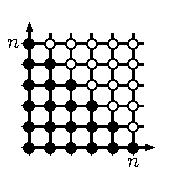
\includegraphics{/Users/zechen/Documents/PrivateAcademic/Analysis/GeneralPointSetTopology/src/graph1.pdf} 
  \end{minipage}
  \begin{proof}
    参考上图,
    \[ C_n = A_n B_n - \leftidx{^{n}_{n}}Ba_1 - \leftidx{^{n}_{n-1}}Ba_2 - \cdots - \leftidx{^{n}_{1}}Ba_n. \]
    由于$\curb{B_n}$为Cauchy列,可以选取$M$使得$n\ge m\ge M$时有$\leftidx{^n_m}B<\epsilon$,
    \[ \abs{C_n-A_nB_n} \le \epsilon\sum\abs{a_n} + \max_{i<M}\abs{B_i}\pare{a_{n-M} + \cdots + a_n}. \qedhere \]
  \end{proof}

  \subsection{级数重排}
  \begin{definition}
    设$\func{f}{\Z_+}{\Z_+}$为双射,则$\sum a_{f\pare{n}}$为$\sum a_n$的重排。
  \end{definition}
  \begin{theorem}
    对于收敛而非绝对收敛的级数和任意$-\infty\le\alpha\le\beta\le+\infty$,存在重排满足$\inf s'_n=\alpha$而$\sup s'_n=\beta$。
  \end{theorem}
  \begin{proof}
    正负分出来,正项累加到刚好过$\alpha$,累加负项到刚好低于$\beta$,循环。
  \end{proof}
  \begin{theorem}
    绝对收敛的级数其任意重排收敛。
  \end{theorem}
  \section{连续函数}
  \subsection{函数的极限}
  \begin{definition}
    谓$\lim_{x\rightarrow p}f\pare{x} = q$,如果对于任意$\epsilon>0$,存在$\delta>0$满足$0 < d\pare{x,p} < \delta \Rightarrow d\pare{f\pare{x},q}<\epsilon$。
  \end{definition}
  \begin{theorem}[\tcompare{matricscontineq}]
    前开定义等价于$p_n\rightarrow p\Rightarrow f\pare{p_n}\rightarrow f\pare{p}$,其中$p_n\neq p$。
  \end{theorem}
  \begin{proof}
    如果定义成立,则显然。若定义不成立,可反证。
  \end{proof}
  \begin{corollary}
    如果$f$在$p$处的极限存在,则极限唯一。
  \end{corollary}
  \begin{theorem}
    若$f\pare{x\rightarrow p}=A$,$g\pare{x\rightarrow p}=B$,则$\pare{f\star g}\pare{x\rightarrow p}=A\star B$。其中$\star$为任意四则运算,对除法假设$B=0$。
  \end{theorem}
  \begin{definition}[连续性的$\epsilon$-$\delta$定义]
    谓$f$在$p$处连续,如果对任意$\epsilon>0$,总存在$\delta>0$满足$d\pare{x,p}<\delta\Rightarrow d\pare{f\pare{x},f\pare{p}}<\epsilon$。
  \end{definition}
  \begin{theorem}[\tcompare{matricscontineq}]
    定义等价于$x\rightarrow p\Rightarrow f\pare{x\rightarrow p}=f\pare{p}$。
  \end{theorem}
  \begin{theorem}[\tcompare{continauscontin}]
    (在某点)连续函数的复合函数仍然连续。
  \end{theorem}
  \begin{theorem}[\tcompare{contineqdeltaepsilon}]
    连续性等价于$V$为开$\Rightarrow \inv{f}\pare{V}$为开。
  \end{theorem}
  \begin{theorem}[\tcompare{contineq}]
    连续性等价于$V$为闭$\Rightarrow \inv{f}\pare{V}$为闭。
  \end{theorem}
  \begin{theorem}[\tcompare{continasmd}]
    连续函数的加减乘除(在非零部分)连续。
  \end{theorem}
  \begin{theorem}[\tcompare{continprod}]
    连续函数的有限Cartesian乘积连续。
  \end{theorem}
  \begin{ex}
    投射、单项式以及定义域内的有理函数连续。
  \end{ex}
  \subsection{连续性和紧性}
  \begin{definition}
    映入$\R^k$的函数谓有界的,如果其像集有界。
  \end{definition}
  \begin{theorem}[\tcompare{imagecompact}]
    紧致度量空间的连续像紧致。
  \end{theorem}
  \begin{theorem}
    紧致度量空间上的连续函数有界。
  \end{theorem}
  \begin{theorem}[\tcompare{extreme}]
    紧度量空间上的连续实函数可取得最值。
  \end{theorem}
  \begin{theorem}[\tcompare{compacthomo}]
    \label{thm:invofcompactcontin}
    紧度量空间到度量空间的双射之逆连续。
  \end{theorem}
  \begin{definition}[\dcompare{unifcontin}]
  一致连续的定义。
  \end{definition}
  \begin{definition}[\tcompare{compactunifcontin}]
    紧度量空间上的连续函数一致连续。
  \end{definition}
  \begin{proof}
    选取$p_n\rightarrow q_n$而$\abs{f\pare{p_n}-f\pare{q_n}}>\epsilon$矛盾。
  \end{proof}
  \begin{theorem}
    若$E$为$\R$中非紧的集,则
    \begin{cenum}
      \item 存在在$E$连续而非有界的函数;
      \item 存在在$E$上连续有界而无最大值的函数;
      \item 若$E$有界,则存在$E$上连续而非一致连续的函数。
    \end{cenum}
  \end{theorem}
  \begin{proof}
    在极限点处做文章即可。
  \end{proof}
  \begin{ex}
    \tref{invofcompactcontin}中紧性不可缺少,\eref{01tocircle}即是一例。
  \end{ex}
  \subsection{连续性与连通性}
  \begin{theorem}[\tcompare{connectcontin}]
    连通空间的连续像是连通的。
  \end{theorem}
  \begin{theorem}[\tcompare{interv}]
    介值定理。
  \end{theorem}
  \subsection{间断}
  \begin{definition}
    $\curb{t_n>x}\Rightarrow f\pare{t_n\rightarrow x} = q$,则谓$f\pare{x+}=q$。类似有$f\pare{x-}$。
  \end{definition}
  \begin{definition}
    谓第一类间断者,$f\pare{x\pm}$皆存在而不等。否则谓第二类。
  \end{definition}
  注意$f\pare{x}$可能等于或不等于$f\pare{x\pm}$。
  \begin{ex}
    $\chi_\Q$在每个点发生第二类间断。
  \end{ex}
  \begin{ex}
    $x\chi_\Q$在$x=0$连续,其他点发生第二类间断。
  \end{ex}
  \begin{ex}
    $f\pare{x}=\sin 1/x \otw 0$在$x=0$处发生第二类间断。
  \end{ex}
  \subsection{单调函数}
  \begin{definition}
    若$x<y\Rightarrow f\pare{x}\le f\pare{y}$则谓之单调递增,类似有单调递减。
  \end{definition}
  \begin{theorem}
    设$\func{f}{\pare{a,b}}{\R}$单调递增,则下列极限存在且
    \[ \sup_{a<t<x} f\pare{t} = f\pare{x-} \le f\pare{x}\le f\pare{x+}=\inf_{x<t<b} f\pare{t}. \]
  \end{theorem}
  \begin{corollary}
    单调函数没有第二类间断。
  \end{corollary}
  \begin{theorem}
    单调函数最多只有可数间断。
  \end{theorem}
  \begin{theorem}
    对于给定的可数集$\curb{x_n}$,存在函数恰好在其上间断,其他地方连续。
  \end{theorem}
  \begin{proof}
    选取收敛的正项级数$\sum c_n$后取
    \[ f= \sum_{x_n<x} c_n. \qedhere \]
  \end{proof}
  \subsection{无穷远处的极限}
  \begin{definition}
    $+\infty$的邻域谓形如$\pare{c,+\infty}$的区间。
  \end{definition}
  \begin{definition}
    设$A$在广义实数系中,若对$A$的邻域$U$皆存在$x$的邻域$V$满足$f\pare{V}\subset U$,则谓$f\pare{t\rightarrow x} = A$。
  \end{definition}
  \begin{theorem}
    函数极限的四则运算在广义实数系内仍然成立。
  \end{theorem}
  注意广义实数系可视为$\R$的两点紧致化。
%ContentEnds
 
\ifx\allfiles\undefined %如果位置放错,可能出现意外中断
\end{document}
\fi
